%% Journal of Open Research Software Latex template -- Created By Stephen Bonner and John Brennan, Durham Universtiy, UK.

\documentclass{jors}

%% Set the header information
\pagestyle{fancy}
\definecolor{mygray}{gray}{0.6}
\renewcommand\headrule{}
\rhead{\footnotesize 3}
\rhead{\textcolor{gray}{UP JORS software Latex paper template version 0.1}}

\begin{document}

{\bf Software paper for submission to the Journal of Open Research Software} \\

To complete this template, please replace the blue text with your own. The paper has three main sections: (1) Overview; (2) Availability; (3) Reuse potential. \\

Please submit the completed paper to: editor.jors@ubiquitypress.com

\rule{\textwidth}{1pt}

\section*{(1) Overview}

\vspace{0.5cm}

\section*{Title}

STAM: Stand-off Text Annotation Model

\section*{Paper Authors}

1. van Gompel, Maarten

\section*{Paper Author Roles and Affiliations}

1. Digital Infrastructure, Humanities Cluster, Royal Netherlands Academy of Arts and Sciences (KNAW)

\section*{Abstract}

We present STAM, a data model with accompanying software for stand-off
annotation on text. The text is treated as a given, i.e. plain text unicode,
devoid of any special markup. Annotations target fragments of the text via
character offsets. Any further annotation paradigm decisions and vocabulary are
up to the user. STAM aims to provide a generic and flexible foundation
with efficient tooling. We implement all the low-level logic needed for
high-performant computation on annotations, allowing you to reuse this and
focus on higher-level applications for researchers.

\section*{Keywords}

annotation; text; computational linguistics; natural language processing

\section*{Introduction}

An \emph{annotation} can be defined as any kind of remark, classification, or
tagging on any particular portion(s) of a text, on the text resource or on
higher-levels such as annotations on annotations, or on the dataset as a whole.
Annotation is the central notion in STAM, the data model we present here. In STAM,
almost everything is expressed via an annotation.

The nature of this annotation is not prescribed in any way, it can be
linguistic, stylistic, structural, editorial, or anything you can think of. We
do not prescribe any vocabulary but offer the wider framework which allows the
user to adopt whatever vocabulary or paradigm they desire. The only premise we
assume is that we are dealing with a piece of structured data that is
associated, directly on indirectly, with text in a \emph{stand-off} fashion.

\emph{Stand-off} annotation decouples annotations from that what is being
annotated. It can be contrasted with in-line annotation such as embodied for
example in mark-up formats like HTML. 

STAM is a two-sided solution; on the one hand it is a data model, this data
model is described in a formal specification fully independent of any implementation.
However, a theoretical model without practical tooling is useless. So on the
other hand STAM comes with dedicated software that implements this model and
allows users to work with it.

We are addressing several fundamental problems that often arise in dealing with annotation:

* How to model annotations  ...?
    * ... as generically as possible? We want to retaining maximum flexibility for the user and separate our model from the semantics of any annotation paradigm or vocabulary.
    * ... as simple as possible? Our data model must be easy to understand for a user/developer to use and only contain what is needed, not more.
* How to efficiently encode annotations... ?
   * ... with respect to space constraints? i.e. avoiding unnecessary duplication and conserving memory.
   * ... with respect to time constraints? i.e. quick (de)serialisation, lookups, searches
* How to efficiently search and retrieve annotations?
    * ... based on annotation data (key/value pairs)
    * ... based on spatial relationships between annotations (e.g. overlap, embedding, adjacency, proximity)
* How to efficiently compute with annotations ... ?
    * ... shifting from absolute offsets to relative offsets within a certain frame of reference?
    * ... verify if certain spatial relationships hold?
* How to safeguard the integrity of annotations?
    * ... ensuring the text which is being pointed at doesn't change?
    * ... ensuring annotations that point at others don't change?
* How to allow easy import and export of data ... ? 
    * .. supporting a variety of accessible serialisation formats such as JSON and CSV, without being strongly bound to any of them.
    * .. import and export from existing models as TEI (XML), FoLiA (XML), and W3C Web Annotations (RDF/JSON-LD).
    * .. retaining also the ability to use high-performance binary serialisation formats?
* How to provide a practical API for annotation?
* How to limit dependencies on further infrastructure, other data models, and other software?

STAM is our answer to these questions. The name STAM is an acronym for
"Stand-off Text Annotation Model". It is Dutch, Swedish, Afrikaans and Frisian for
"trunk" (as in the trunk of a tree), the name represents a solid foundation
upon which one can build.

In the same spirit, the software we built for STAM caters towards an audience
of developers and technically-skilled researchers. We deliver fairly low-level
programming libraries and command-line tools that may serve as dependencies for
higher-level applications. 

Last but not least, it prevents misunderstanding to make clear what STAM is
\emph{not}: STAM is \emph{not} a graphical user interface for annotation, it is
\emph{not} a natural language processing tool for producing annotations, and it
is \emph{not} a specific vocabulary for any particular class of annotation. It
may be a foundation for any of those things though. It is also \emph{not}
intended as a replacement for existing dedicated annotation formats, but more
of a complement to those to allow further computation and processing.

\textcolor{blue}{An overview of the software, how it was produced, and the
research for which it has been used, including references to relevant research
articles. A short comparison with software which implements similar
functionality should be included in this section. }

\section*{Implementation and architecture}

\subsection*{Data Model}

The data model for STAM can be subdivided into a \emph{core model}, an
\emph{extended model}, and multiple \emph{extensions}. The core model defines
data concepts that are all required in any STAM implementation. The extended
model is closely related and adds some concepts that implementations may
deviate from. Last, the extensions are each separately formulated
specifications that add specific but optional functionality that users may or
may not use, and implementations may or may not implement. We chose this setup
to keep things as minimal, modular and maintainable as possible.

In Figure~\ref{fig:modelintro} we introduce the core model schematically in a
bottom-up fashion. All of the concepts from the core or extended model are
marked in bold in this section. We start with the central notion of
\textbf{annotation}. In the left branch we see \emph{what} the annotations
says, and in the right branch we see \emph{about what} the annotation says
something. The left is expressed via \textbf{annotation
data}, which is in turn made up of a \textbf{data key} and \textbf{data value} pair.
The right is expressed via the core concept of a \textbf{selector}, which
describes the target of the annotation.

\begin{figure}[h]
\includegraphics{../presentation/slide3b.png}
\caption{Schematic illustration of a STAM annotation on a small piece of text.}
\label{fig:modelintro}
\end{figure}

STAM defines a number of selectors, Figure~\ref{fig:modelintro} shows one of
the most common ones, the \textbf{text selector}, which targets a portion of a
text (a so-called \textbf{text selection}). This is done via a reference to the
\textbf{text resource} as a whole and to a specific \textbf{offset} within the
text. An offset consists of two \textbf{cursors}, one pointing at the start,
and one pointing at the end. The coordinate system is strictly defined by STAM,
follows unicode character points, is zero-indexed and the end is always
non-inclusive.

The figure illustrates how the last word in the Swedish phrase \emph{``Hallå
världen''} is being annotated. The annotation links the word \emph{``världen''}
in the text with the annotation data that says it is a noun. That is, it gets
annotated with data key \emph{``pos''} (part-of-speech) and data value
\emph{``noun''}. This vocabulary is wholly fictitious and in no way predefined
by STAM. 

The vocabulary is completely up to the user. Vocabulary is kept in an
\textbf{annotation dataset}. The data set holds the annotation data (i.e. the
keys and the values).\footnote{The annotation data actually holds the data values, but
makes reference to the data keys, which is held seperately in the annotation
dataset.}. An annotation may reference multiple annotation data rather than
just one, and the annotation data may be from multiple sets.

Two more things can be discerned in the schema. First, many core concepts in
STAM, such as annotations, annotation data, annotation dataset and text
resources may carry a \textbf{public identifier}, which can be any kind of
string. Second, we can see that data values are typed; STAM defines
a few elementary types (e.g. string, integer, float, date/time).

A text selection is by definition contiguous (described by a single offset) in
STAM. This, however, does not offer enough expressibility. To annotate
discontinuous text fragments we introduce \textbf{complex selectors} such as
the \textbf{composite selector}. This selector may in turn hold multiple (non-complex)
selectors. It allows selecting multiple text selections, as a joint composition,
from a single annotation. Figure~\ref{fig:modelintro2} illustrates this
schematically.

\begin{figure}[h]
\includegraphics{../presentation/slide3e.png}
\caption{An annotation of a Dutch split verb using a composite selector. The annotation associates a single lemma with the split verb.}
\label{fig:modelintro2}
\end{figure}

In STAM, almost everything is an annotation. Rather than annotate text
directly, we may choose to annotate it indirectly by pointing at other
annotations. This is accomplished via an \textbf{annotation selector}. We may
also annotate not the actual text but the resource or data set as a whole via a
\textbf{resource selector} or \textbf{dataset selector}. This effectively makes
for a kind of metadata annotation and may be useful for annotation such as
expressing who the author of a resource was, or what the license is.

In Figure~\ref{fig:modelintro3} we take a more top-down perspective at how data
is organized in the core STAM model. At the top-level we have the notion of an
\textbf{annotation store}, which is essentially the workspace that
holds the annotations. It also holds the \textbf{annotation datasets} (and by
extension the \textbf{annotation data}), and the \textbf{text resources},
but both of these may be stored stand-off and need not be unique to a single
annotation store.

\begin{figure}[h]
\includegraphics{../presentation/slide3e.png}
\caption{A top down overview of the way data is organized in the STAM model}
\label{fig:modelintro3}
\end{figure}

STAM defines a canonical serialisation format using JSON that maps the all the
core concepts pretty directly to a verbose JSON representation, which is aptly
called STAM JSON. The user has the choice whether to serialize annotation data
sets and text resources (as plain text) independently, or to include them in a
single STAM JSON serialisation. JSON is used only here as an easy way to get
data in an out, and chosen because of its ubiquity. But it is verbose and does not
pretend to be optimal in any way.

At this point, we discussed most of the model. We refer to the
specification for the full details, which also includes detailed UML diagrams.

What remains is the extensions. It is out of scope to go into much detail here,
we will merely list the extensions that are currently formulated and
implemented:

\begin{itemize}
\item \textbf{STAM Vocab} - Allows expressing and validating against user-defined vocabularies.
\item \textbf{STAM WebAnnotation} - Expresses STAM model using W3C Web Annotations (and vice versa), this also implies it expresses RDF and provides the gateway for STAM to integrate with the world of linked open data.
\item \textbf{STAM Textvalidation} - Adds an extra redundancy layer that helps protecting data integrity and aids readability of serialisations.
\item \textbf{STAM CSV} - Defines an alternative serialisation format using CSV.
\item \textbf{STAM Query Language (STAMQL)} - This STAM extension defines a query language that allows end-users to formulate and subsequently execute searches on a STAM model.
\item \textbf{STAM Transpose} - This is an extension on top of STAM that allows linking identical textual parts across resources, which we call transposition. This extension defines a vocabulary and prescribes functionality enabled through this vocabulary.
\end{itemize}

\subsection*{Software}

The STAM specification defines what functionality implementations must provide
in order to be considered full implementations of STAM, but it also still
leaves a lot of freedom for developers to decide how to implement things.  The
aim for our reference implementation was to deliver a potent software library
with an API that allows users to add, retrieve and search annotations. Our
criteria and considerations were:

\begin{itemize}
    \item The library must be performant and reliable, we therefore chose to implement it in Rust, as that compiles to native code with memory-safety guarantees.
    \item Our main aim is to be able to efficiently search and compute on annotations, we therefore opted for an implementation that is largely memory-based.
    \item The library must not rely on any further service infrastructure but be fairly standalone and fully usable also on a local non-networked machine. It therefore does not rely on things like a database server.
    \item To make it accessible for higher-level developers and technically-skilled researchers and data scientists, we implement a Python binding on top of the Rust library. This combines the best of both worlds.
    \item Moreover, we also provide command-line tools. These also add functionality that is not in the main library, but defined in the STAM extensions.
    \item Everything that is formulated as an extension and still implemented in the main Rust library can be disabled at compile time.
\end{itemize}

The typical workflow is to load a STAM annotation store from disk (e.g. from
STAM JSON) into memory, operate on the annotations, and serialize the data to
disk again if any changes were made.

Our approach can be contrasted to implementations that would store the data in
a relational database, or any other kind of database engine, and load into
memory only parts when needed. This too would be a feasible way of implementing
STAM. It would, however, be subject to greater latency. There is a trade-off
between low-latency and high-scalability. Our current implementation
deliberately tends towards the former rather than the latter. Our
implementation is also sufficiently optimised to allow working with millions of
annotations without running into memory issues.

Internally, various reverse indices are built to facilitate data retrieval.

%Conceptually, a STAM model can be conceived of as an acyclic directed graph, in
%which the annotations, annotation data, data keys, data values and text
%resources are all nodes and the links between them edges. This is also strongly
%reflected in the memory ownership model of the Rust implementation.



%TODO: documentation


\textcolor{blue}{How the software was implemented, with details of the
architecture where relevant. Use of relevant diagrams is appropriate. Please
also describe any variants and associated implementation differences.}

\section*{Quality control}

Building a solid library was one of the main goals, so testing is major 
aspect of that. Many unit and integration tests have been implemented and
automatically run on a continuous integration platform.

A certain amount of quality is also assured to due to the choice of
language. The use of Rust prevents a wide class of errors that are common in
other system programming languages like C and C++, mostly related to memory
management.






\textcolor{blue}{Detail the level of testing that has been carried out on the
code (e.g. unit, functional, load etc.), and in which environments. If not
already included in the software documentation, provide details of how a user
could quickly understand if the software is working (e.g. providing examples of
running the software with sample input and output data). }

\section*{(2) Availability}
\vspace{0.5cm}
\section*{Operating system}

The stam library for Rust compiles on all 64-bit architectures where a Rust compiler (version 1.56 or later, edition 2021) is available.
A simple \texttt{cargo add stam} suffices to add it to your own Rust project.

For the Python binding, Python wheel packages are provided via the Python Package Index for Linux (x86_64/arm64, glibc/musl), macOS (x86_64/arm64) and Windows (x86_64).
A simple \texttt{pip install stam} suffices in most cases.

\section*{Programming language}

A Rust installation is not needed if you use the Python binding or the command-line tools and if it is packaged for your distribution.

The Python binding requires Python 3.7 or later. 

\textcolor{blue}{Please include minimum version compatibility.}

\section*{Additional system requirements}

The implementation is memory-based, so the amount of annotations and texts you can load at the same time will be bound by available memory. A minimum memory recommentation for medium-size text collections is 6GB.

For certain computations, the STAM library may use parallellization and thus benefits from multiple CPU cores.

The command-line tools work best with a POSIX-compliant unix shell like bash or zsh. Windows shells are less tested and may face limitations. 

\textcolor{blue}{E.g. memory, disk space, processor, input devices, output devices.}

\section*{Dependencies}

None aside from compile-time dependencies for the Rust library/tools, all binaries are statically linked.

Python for the Python binding, a shell for the command line tools, and a supported libc version.

\section*{List of contributors}

\textcolor{blue}{Please list anyone who helped to create the software (who may also not be an author of this paper), including their roles and affiliations.}

\section*{Software location:}

{\bf Archive} \textcolor{blue}{(e.g. institutional repository, general repository) (required – please see instructions on journal website for depositing archive copy of software in a suitable repository)} 

\begin{description}[noitemsep,topsep=0pt]
	\item[Name:] \textcolor{blue}{The name of the archive.}
	\item[Persistent identifier:] \textcolor{blue}{e.g. DOI, handle, PURL, etc.}
	\item[Licence:] \textcolor{blue}{Open license under which the software is licensed.}
	\item[Publisher:]  \textcolor{blue}{Name of the person who deposited the software.}
	\item[Version published:] \textcolor{blue}{The version number of the software archived.}
	\item[Date published:] \textcolor{blue}{dd/mm/yy}
\end{description}



{\bf Code repository} \textcolor{blue}{(e.g. SourceForge, GitHub etc.) (required)}

\begin{description}[noitemsep,topsep=0pt]
	\item[Name:] \textcolor{blue}{The name of the archive.}
	\item[Persistent identifier:] \textcolor{blue}{e.g. DOI, handle, PURL, etc.}
	\item[Licence:] \textcolor{blue}{Open license under which the software is licensed.}
	\item[Date published:] \textcolor{blue}{dd/mm/yy}
\end{description}

{\bf Emulation environment} \textcolor{blue}{(if appropriate)}

\begin{description}[noitemsep,topsep=0pt]
	\item[Name:] \textcolor{blue}{The name of the archive.}
	\item[Persistent identifier:] \textcolor{blue}{e.g. DOI, handle, PURL, etc.}
	\item[Licence:] \textcolor{blue}{Open license under which the software is licensed.}
	\item[Date published:] \textcolor{blue}{dd/mm/yy}
\end{description}

\section*{Language}

English

\section*{(3) Reuse potential}

\textcolor{blue}{Please describe in as much detail as possible the ways in which the software could be reused by other researchers both within and outside of your field. This should include the use cases for the software, and also details of how the software might be modified or extended (including how contributors should contact you) if appropriate. Also you must include details of what support mechanisms are in place for this software (even if there is no support).}

\section*{Acknowledgements}

\textcolor{blue}{Please add any relevant acknowledgements to anyone else who supported the project in which the software was created, but did not work directly on the software itself.}

\section*{Funding statement}

\textcolor{blue}{If the software resulted from funded research please give the funder and grant number.}

\section*{Competing interests}

\textcolor{blue}{If any of the authors have any competing interests then these must be declared. The authors’ initials should be used to denote differing competing interests. For example: “BH has minority shares in [company name], which part funded the research grant for this project. All other authors have no competing interests." \\
If there are no competing interests, please add the statement:
“The authors declare that they have no competing interests.” }

\section*{References}

\textcolor{blue}{Please enter references in the Harvard style and include a DOI where available, citing them in the text with a number in square brackets, e.g. \\ }

\textcolor{blue}{[1] Piwowar, H A 2011 Who Shares? Who Doesn't? Factors Associated with Openly Archiving Raw Research Data. PLoS ONE 6(7): e18657. DOI: \\ http://dx.doi.org/10.1371/journal.pone.0018657.}

\vspace{2cm}

\rule{\textwidth}{1pt}

{ \bf Copyright Notice} \\
Authors who publish with this journal agree to the following terms: \\

Authors retain copyright and grant the journal right of first publication with the work simultaneously licensed under a  \href{http://creativecommons.org/licenses/by/3.0/}{Creative Commons Attribution License} that allows others to share the work with an acknowledgement of the work's authorship and initial publication in this journal. \\

Authors are able to enter into separate, additional contractual arrangements for the non-exclusive distribution of the journal's published version of the work (e.g., post it to an institutional repository or publish it in a book), with an acknowledgement of its initial publication in this journal. \\

By submitting this paper you agree to the terms of this Copyright Notice, which will apply to this submission if and when it is published by this journal.


\end{document}
